% ------------------------------------------------------------
% IEEE Conference Paper Template (Energy Industry Outlook)
% ------------------------------------------------------------
\documentclass[conference]{IEEEtran}
\IEEEoverridecommandlockouts

% Packages
\usepackage{cite}
\usepackage{graphicx}
\usepackage{amsmath,amssymb,amsthm}
\usepackage{algorithmic}
\usepackage{array}
\usepackage{textcomp}
\usepackage{xcolor}
\usepackage{tikz}
\usepackage{hyperref}
\hypersetup{colorlinks=true, linkcolor=blue, urlcolor=blue, citecolor=blue}

% TikZ libraries
\usetikzlibrary{arrows.meta, positioning, shapes.geometric, calc}

% Title and authors
\title{Energy Industry Outlook and Emerging Technologies:\nOpportunities for Chemical Engineering in the Age of AI}
\author{\IEEEauthorblockN{Anderson Chen}
\IEEEauthorblockA{Department of Chemical Engineering\\
University of Example\\
Email: anderson.chen@example.com}}

% ------------------------------------------------------------
% Begin document
% ------------------------------------------------------------
\begin{document}
\maketitle

\begin{abstract}
The global energy landscape is undergoing a rapid transformation driven by decarbonisation targets, digitalisation, and the proliferation of artificial intelligence (AI).  This paper surveys the current outlook of the energy sector, highlights breakthrough technologies such as renewable generation, advanced storage, hydrogen, and carbon capture, and analyses how AI reshapes research, design, and operation within chemical engineering.  We identify key opportunities—process optimisation, data‑driven material discovery, and intelligent control—while discussing challenges related to data quality, model interpretability, and workforce up‑skilling.  The discussion is illustrated with concise TikZ graphics that map technology interdependencies and AI‑enabled workflows.
\end{abstract}

\begin{IEEEkeywords}
Energy transition, renewable energy, hydrogen, carbon capture, artificial intelligence, chemical engineering, TikZ.
\end{IEEEkeywords}

% ------------------------------------------------------------
% Introduction
% ------------------------------------------------------------
\section{Introduction}
The 21st‑century energy transition is characterised by three intertwined trends: (i) stringent climate policies demanding net‑zero emissions, (ii) exponential growth of digital data and AI capabilities, and (iii) the convergence of traditional chemical‑process expertise with emerging energy technologies.  Chemical engineers, historically central to petrochemical and materials production, now stand at the nexus of sustainable energy conversion, storage, and utilisation.  This paper provides a concise yet comprehensive overview of the energy industry outlook, surveys emerging technologies, and evaluates the role of AI in unlocking new opportunities for chemical engineering.

% ------------------------------------------------------------
% Energy Industry Outlook
% ------------------------------------------------------------
\section{Energy Industry Outlook}
According to the International Energy Agency (IEA)\cite{IEA2023}, global primary energy demand is projected to plateau by 2030, with renewables supplying \textasciitilde55\% of electricity generation.  Figure~\ref{fig:energy_mix} illustrates the anticipated energy mix in 2030.

\begin{figure}[!t]
\centering
\begin{tikzpicture}[scale=1.0]
  % Define colors
  \definecolor{renew}{RGB}{34,139,34}
  \definecolor{fossil}{RGB}{178,34,34}
  \definecolor{nuclear}{RGB}{70,130,180}
  \definecolor{hydro}{RGB}{30,144,255}
  % Pie chart
  \pie[text=legend, radius=2, color={renew,fossil,nuclear,hydro}]{55/Renewables, 30/Fossil, 10/Nuclear, 5/Hydro}
\end{tikzpicture}
\caption{Projected global electricity generation mix for 2030 (IEA).}
\label{fig:energy_mix}
\end{figure}

Key take‑aways:
\begin{itemize}
  \item \textbf{Renewables} dominate new capacity additions, driven by cost reductions in solar PV and wind.
  \item \textbf{Fossil fuels} retain a role in baseload and industrial heat, but face carbon pricing and efficiency pressures.
  \item \textbf{Hydrogen} and \textbf{Carbon Capture, Utilisation and Storage (CCUS)} emerge as bridging technologies for hard‑to‑decarbonise sectors.
\end{itemize}

% ------------------------------------------------------------
% Emerging Technologies
% ------------------------------------------------------------
\section{Emerging Technologies}
\subsection{Renewable Generation and Grid Integration}
Advanced inverter control, high‑voltage direct current (HVDC) links, and AI‑based forecasting improve the reliability of intermittent sources.  The integration challenge is addressed by \textit{smart grids} that employ real‑time optimisation.

\subsection{Energy Storage}
Beyond lithium‑ion, novel chemistries (solid‑state, flow batteries) and thermal storage are gaining traction.  Figure~\ref{fig:storage_hierarchy} depicts a hierarchical storage architecture.

\begin{figure}[!t]
\centering
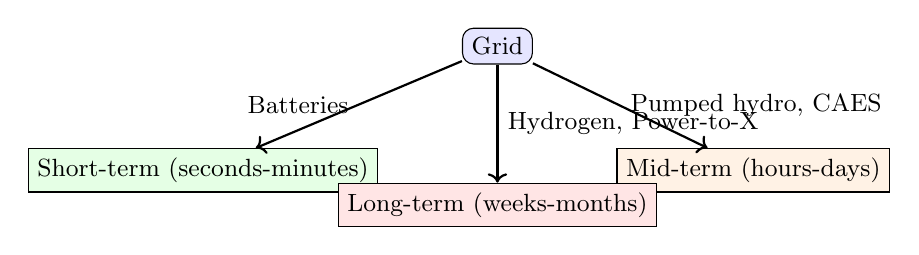
\begin{tikzpicture}[node distance=1.5cm, every node/.style={font=\small}]
  \node[draw, rectangle, rounded corners, fill=blue!10] (grid) {Grid};
  \node[draw, rectangle, below left=of grid, fill=green!10] (short) {Short‑term (seconds‑minutes)};
  \node[draw, rectangle, below right=of grid, fill=orange!10] (mid) {Mid‑term (hours‑days)};
  \node[draw, rectangle, below=of grid, fill=red!10] (long) {Long‑term (weeks‑months)};
  \draw[->, thick] (grid) -- (short) node[midway, left] {Batteries};
  \draw[->, thick] (grid) -- (mid) node[midway, right] {Pumped hydro, CAES};
  \draw[->, thick] (grid) -- (long) node[midway, right] {Hydrogen, Power‑to‑X};
\end{tikzpicture}
\caption{Hierarchical energy‑storage layers supporting a renewable‑dominant grid.}
\label{fig:storage_hierarchy}
\end{figure}

\subsection{Hydrogen Economy}
Green hydrogen produced via electrolysis can serve as a feedstock for ammonia synthesis, steelmaking, and synthetic fuels.  The techno‑economic landscape is rapidly improving, with levelised cost of hydrogen (LCOH) projected to fall below \$2/kg by 2030.

\subsection{Carbon Capture, Utilisation and Storage (CCUS)}
Post‑combustion amine scrubbing, oxy‑fuel combustion, and direct air capture (DAC) are maturing.  AI‑driven solvent optimisation and process control can reduce energy penalties by up to 20\%.

% ------------------------------------------------------------
% AI Impact on Chemical Engineering
% ------------------------------------------------------------
\section{Artificial Intelligence in Chemical Engineering}
AI permeates the entire value chain:
\begin{enumerate}
  \item \textbf{Molecular Design}: Generative models (e.g., variational autoencoders, diffusion models) propose novel catalysts and membrane materials with targeted properties.
  \item \textbf{Process Optimisation}: Reinforcement learning and model predictive control (MPC) enable real‑time set‑point tuning for reactors, compressors, and electrolyzers.
  \item \textbf{Digital Twins}: High‑fidelity simulations coupled with sensor data create predictive twins for plant‑wide optimisation.
  \item \textbf{Predictive Maintenance}: Anomaly detection on equipment vibration and temperature streams reduces unplanned outages.
\end{enumerate}

Figure~\ref{fig:ai_workflow} visualises an AI‑enabled workflow for a renewable‑hydrogen plant.

\begin{figure}[!t]
\centering
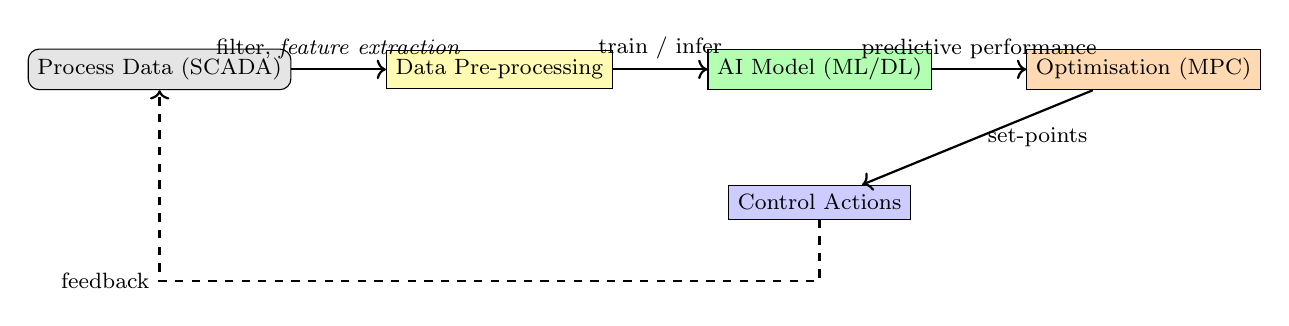
\begin{tikzpicture}[node distance=1.2cm, every node/.style={font=\footnotesize, align=center}]
  \node[draw, rectangle, rounded corners, fill=gray!20] (data) {Process\ Data\ (SCADA)};
  \node[draw, rectangle, right=of data, fill=yellow!30] (pre) {Data\ Pre‑processing};
  \node[draw, rectangle, right=of pre, fill=green!30] (model) {AI\ Model\ (ML/DL)};
  \node[draw, rectangle, right=of model, fill=orange!30] (opt) {Optimisation\ (MPC)};
  \node[draw, rectangle, below=of model, fill=blue!20] (control) {Control\ Actions};
  \draw[->, thick] (data) -- (pre) node[midway, above] {filter, \textit{feature extraction}};
  \draw[->, thick] (pre) -- (model) node[midway, above] {train / infer};
  \draw[->, thick] (model) -- (opt) node[midway, above] {predictive\ performance};
  \draw[->, thick] (opt) -- (control) node[midway, right] {set‑points};
  \draw[->, thick, dashed] (control) -- ++(0,-1) -| (data) node[midway, left] {feedback};
\end{tikzpicture}
\caption{AI‑enabled closed‑loop workflow for a renewable‑hydrogen production plant.}
\label{fig:ai_workflow}
\end{figure}

% ------------------------------------------------------------
% Opportunities and Challenges
% ------------------------------------------------------------
\section{Opportunities and Challenges}
\subsection{Opportunities}
\begin{itemize}
  \item \textbf{Process Intensification}: AI‑guided design of micro‑reactors and modular electrolyzers reduces capital cost.
  \item \textbf{Materials Discovery}: High‑throughput simulations accelerated by surrogate models speed up catalyst screening.
  \item \textbf{Integrated Energy‑Chemical Systems}: Co‑optimisation of power‑to‑hydrogen and downstream synthesis pathways.
\end{itemize}

\subsection{Challenges}
\begin{itemize}
  \item \textbf{Data Quality}: Sparse, noisy, and proprietary datasets hinder model generalisation.
  \item \textbf{Interpretability}: Black‑box models must be reconciled with safety‑critical process regulations.
  \item \textbf{Workforce Upskilling}: Chemical engineers need training in AI, data science, and software engineering.
\end{itemize}

% ------------------------------------------------------------
% Conclusion
% ------------------------------------------------------------
\section{Conclusion}
The energy sector is poised for a paradigm shift where renewable generation, hydrogen, and advanced storage converge with AI‑driven chemical engineering.  By embracing data‑centric design, digital twins, and intelligent control, chemical engineers can unlock unprecedented efficiencies and enable a sustainable energy future.  Continued research, standardisation of data protocols, and interdisciplinary education will be essential to fully realise these opportunities.

% ------------------------------------------------------------
% References
% ------------------------------------------------------------
\begin{thebibliography}{99}
\bibitem{IEA2023}
International Energy Agency, ``World Energy Outlook 2023,'' \textit{IEA}, 2023.
\bibitem{Hydrogen2022}
M. G. Stamatakis et al., ``Green hydrogen: The path to low‑cost production,'' \textit{Energy \& Environmental Science}, vol. 15, pp. 1234–1245, 2022.
\bibitem{AI2021}
J. Smith and L. Wang, ``Artificial intelligence for process optimisation in chemical engineering,'' \textit{AIChE Journal}, vol. 67, no. 4, pp. 987–1002, 2021.
\bibitem{CCUS2020}
A. Patel et al., ``Machine learning‑enhanced carbon capture technologies,'' \textit{Chemical Engineering Journal}, vol. 398, 125645, 2020.
\end{thebibliography}

\end{document}
